\documentclass[a4paper, twocolumn, landscape, 9pt]{article}
\usepackage[utf8]{inputenc}
\usepackage[T1]{fontenc}
\usepackage{multicol}
\usepackage[margin=0.5in, bmargin=0.4in, tmargin=0.8in]{geometry}
\usepackage{titlesec}
\usepackage{graphicx}
\usepackage{etoolbox}
\usepackage{fancyhdr}
\usepackage[titles]{tocloft}
\usepackage{listings}
\usepackage{amsmath}
\usepackage{hyperref}

\hypersetup{
  colorlinks,
  citecolor=black,
  filecolor=black,
  linkcolor=black,
  urlcolor=black
}
 
\pagestyle{fancy}
\fancyhf{}
\rhead{Page \thepage}
\lhead{Federal University of Bahia - Universidade Federal da Bahia}

\lstset{
language=R, 
literate=
{≡}{{$\equiv$}}1
{∩}{{$\cap$}}1
{∪}{{$\cup$}}1
{∛N}{{$\sqrt[3]{N}$}}1
{Ã}{{\~A}}1
{Á}{{\'A}}1
{Â}{{\^A}}1
{á}{{\'a}}1
{à}{{\`a}}1
{ã}{{\~a}}1
{â}{{\^a}}1
{é}{{\'e}}1
{É}{{\'E}}1
{ê}{{\^e}}1
{í}{{\'i}}1
{ó}{{\'o}}1
{ô}{{\^o}}1
{õ}{{\~o}}1
{ú}{{\'u}}1
{ü}{{\"u}}1
{ç}{{\c{c}}}1
}

\usepackage{xcolor}
\usepackage{listings}
% \usepackage{courier}
\usepackage{courier}
\usepackage{pgfplotstable}
% recommended:
\usepackage{booktabs}
\usepackage{array}
\usepackage{colortbl}
\usepackage{verbatim}
\usepackage{xstring}

\definecolor{mygreen}{rgb}{0,0.6,0}
\definecolor{mygray}{rgb}{0.5,0.5,0.5}
\definecolor{mymauve}{rgb}{0.58,0,0.82}
\definecolor{codegreen}{rgb}{0,0.6,0}
\definecolor{codegray}{rgb}{0.5,0.5,0.5}
\definecolor{codepurple}{rgb}{0.58,0,0.82}
\definecolor{backcolour}{rgb}{0.95,0.95,0.92}

\def\trim#1{\ignorespaces#1\unskip} 

\lstset{ %
  basicstyle=\linespread{0.82}\footnotesize\ttfamily,        % the size of the fonts that are used for the code
  breakatwhitespace=true,         % sets if automatic breaks should only happen at whitespace
  breaklines=true,                 % sets automatic line breaking
  commentstyle=\itshape\color{black!63},    % comment style
  extendedchars=true,              % lets you use non-ASCII characters; for 8-bits encodings only, does not work with UTF-8
  frame=lbtr,                    % adds a frame around the code
  keepspaces=true,                 % keeps spaces in text, useful for keeping indentation of code (possibly needs columns=flexible)
  keywordstyle=\bfseries,       % keyword style
  numbers=left,                    % where to put the line-numbers; possible values are (none, left, right)
  numbersep=8pt,                   % how far the line-numbers are from the code
  numberstyle=\scriptsize, % the style that is used for the line-numbers
  rulecolor=\color{black},         % if not set, the frame-color may be changed on line-breaks within not-black text (e.g. comments (green here))
  showspaces=false,                % show spaces everywhere adding particular underscores; it overrides 'showstringspaces'
  showstringspaces=false,          % underline spaces within strings only
  showtabs=false,                  % show tabs within strings adding particular underscores
  stringstyle=,     % string literal style
  tabsize=2,                     % sets default tabsize to 2 spaces
  inputencoding=utf8
}

\lstdefinestyle{colored}{
  basicstyle=\footnotesize\ttfamily,
  keywordstyle=\color{green!30!black},
  commentstyle=\itshape\color{purple!40!black},
  identifierstyle=,
  stringstyle=\color{orange},
}

\lstdefinestyle{mystyle}{
  %backgroundcolor=\color{backcolour},   
  commentstyle=\color{green!30!black},
  keywordstyle=\color{magenta},
  numberstyle=\color{codegray},
  stringstyle=\color{codepurple},
  rulecolor=\color{codegray},
}

\lstset{columns=fullflexible}

\def\EOF{1000}

\def\normLineNumber#1{\trim{\detokenize{#1}}}

\newcommand{\includenote}[1]{\lstinputlisting{codes/#1}}
\newcommand{\includecode}[2][C++]{
  \lstinputlisting[escapechar=, language=#1]{codes/#2}
}

\newcommand{\includepiece}[3][C++]{
  %{\detokenize{#2} (\normLineNumber{#3})}
  \lstinputlisting[escapechar=, language=#1, linerange={#3}]{codes/#2}
}

% \pgfplotstabletypeset{col sep=tab}

\newcommand{\includetable}[1]{
  \begin{verbatim}\input{notes/#1}\end{verbatim}
}


% usage of commands
% section, subsection and subsubsection were renewed so they receive 2 arguments instead of 1. ex: \section{title}{text}
% \includecode[language]{file} include code from codes/{file}. default language is C++.
% \includepiece[language]{file}{firstline}{lastline} does the same thing, but it includes from firstline to lastline only.
%

%% Control the fonts and formatting used in the table of contents.

%% Aesthetic spacing redefines that look nicer to me than the defaults.

\setlength{\cftbeforesecskip}{0.02em}
\setlength{\cftbeforesubsecskip}{0.02em}
\setlength{\cftbeforesubsubsecskip}{0.02em}

%% Use Helvetica-Narrow Bold for Chapter entries

\renewcommand{\cftsecfont}{%
  \fontsize{10}{10}\usefont{T1}{phv}{bc}{n}\selectfont
}
\renewcommand{\cftsubsecfont}{
	\fontsize{9}{9}\usefont{T1}{phv}{c}{n}\selectfont
}
\renewcommand{\cftsubsubsecfont}{
	\fontsize{9}{9}\usefont{T1}{phv}{c}{n}\selectfont
}

\renewcommand{\familydefault}{\ttdefault}
\setlength{\columnsep}{1cm}

\let\Asection\section
\let\Bsection\subsection
\let\Csection\subsubsection

\renewcommand{\section}[2]{
   \ifstrequal{#2}{}{\Asection[#1 *]{#1} #2}{\Asection{#1} #2} %
}
\renewcommand{\subsection}[2]{
    \ifstrequal{#2}{}{\Bsection[#1 *]{#1} #2}{\Bsection{#1} #2} %
}
\renewcommand{\subsubsection}[2]{
    \ifstrequal{#2}{}{\Csection[#1 *]{#1} #2}{\Csection{#1} #2} %
}

\title{Competitive Programming Library}
\author{Bernardo Flores Salmeron}
\date{}

\begin{document}
	
\titleformat{\section}[hang]{\large}{}{0pt}{\thesection. }
\titleformat{\subsection}[hang]{\normalsize}{}{0pt}{\thesubsection. }
\titleformat{\subsubsection}[hang]{\small}{}{0pt}{\thesubsubsection. }
\titlespacing{\section}{0px}{3px}{2px}
\titlespacing{\subsection}{0px}{2px}{1px}

% generate title and table of contents with no heading
\maketitle
\thispagestyle{fancy}

\makeatletter
%\renewcommand{\l@subsection}{\@dottedtocline{2}{1.5em}{3.0em}}
%\renewcommand{\l@subsubsection}{\@dottedtocline{3}{3.0em}{4em}}
\def\tableofcontents{\@starttoc{toc}}
\makeatother

% \centering\textcolor{red}{\textbf{THE WHOLE LIB USES dcmp() FOR FLOATING-POINT COMPARISON}}

\tableofcontents
\newpage
\newpage

\section{Template}{
  \includecode{template.cpp}
}

\section{Funcoes Interessantes}{

  \subsection{GCD}{
    \includecode{"Funcoes Interessantes"/GCD.cpp}
  }

  \subsection{HIPOTENUSA}{
    \includecode{"Funcoes Interessantes"/Hipotenusa.cpp}
  }

  \subsection{SCANF DE UMA STRING}{
    \includecode{"Funcoes Interessantes"/"Scanf de uma string".cpp}
  }

  \subsection{PRINTF PARA UMA STRING}{
    \includecode{"Funcoes Interessantes"/"Printf de uma string".cpp}
  }

  \subsection{CLIMITS}{
    \includecode{"Funcoes Interessantes"/CLIMITS.cpp}
  }

  \subsection{ROTATE (LEFT)}{
    \includecode{"Funcoes Interessantes"/"Rotate (Left)".cpp}
  }

  \subsection{ROTATE (RIGHT)}{
    \includecode{"Funcoes Interessantes"/"Rotate (Right)".cpp}
  }

  \subsection{WIDTH}{
    \includecode{"Funcoes Interessantes"/"Width".cpp}
  }

  \subsection{INT TO STRING (C++11)}{
    \includecode{"Funcoes Interessantes"/"Int to String".cpp}
  }

  \subsection{PERMUTAÇÃO}{
    \includecode{"Funcoes Interessantes"/"Permutacao".cpp}
  }

  \subsection{MAIOR E MENOR ELEMENTO NUM VETOR}{
    \includecode{"Funcoes Interessantes"/"Max e Min Element num vetor".cpp}
  }

  \subsection{CHECAGEM E TRANSFORMAÇÃO DE CARACTERE}{
    \includecode{"Funcoes Interessantes"/"Checagem e Tranformacao de Caractere".cpp}
  }

  \subsection{SUBSTRING}{
    \includecode{"Funcoes Interessantes"/"Substring".cpp}
  }

  \subsection{REMOVE REPETIÇÕES CONTÍNUAS NUM VETOR}{
    \includecode{"Funcoes Interessantes"/"Remove Repeticoes Continuas num Vetor".cpp}
  }

  \subsection{CHECAGEM DE BITS}{
    \includecode{"Funcoes Interessantes"/"Checagem de Bits".cpp}
  }

  \subsection{INT TO BINARY STRING}{
    \includecode{"Funcoes Interessantes"/"Int to Binary String".cpp}
  }

  \subsection{BINARY STRING TO INT}{
    \includecode{"Funcoes Interessantes"/"Binary String to Int".cpp}
  }

  \subsection{STRING TO LONG LONG}{
    \includecode{"Funcoes Interessantes"/"String to Long Long".cpp}
  }

  \subsection{SPLIT FUNCTION }{
    \includecode{"Funcoes Interessantes"/"Split Function".cpp}
  }

  \subsection{LEITURA NUM ARQUIVO}{
    \includecode{"Funcoes Interessantes"/"Leitura de Arquivo".cpp}
  }

  \subsection{ESCRITA EM ARQUIVO}{
    \includecode{"Funcoes Interessantes"/"Escrita em Arquivo".cpp}
  }

  \subsection{CHECAGEM BRUTE FORCE COM SOLUCAO}{
    \includecode{"Funcoes Interessantes"/"Checagem Brute Force com Solucao".cpp}
  }    

}

\newpage

\section{DP}{
  \subsection{PROBLEMA DO TROCO}{

    \includecode{DP/troco.cpp}
  }

  \subsection{PROBLEMA DA MOCHILA}{
    \includecode{DP/Knapsack.cpp}
  }

  \subsection{CATALAN (1, 1, 2, 5, 14, 42, 132, 429) - $O(n)$}{
    \centering
    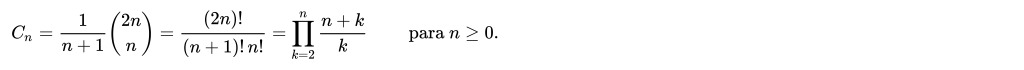
\includegraphics[scale=0.5]{Images/Catalan.jpg}
    \includecode{DP/Catalan.cpp}
  }

  \subsection{LONGEST COMMON SUBSEQUENCE - $O(n^{2})$}{
    \includecode{DP/"Longest Common Subsequence".cpp}
  }

  \subsection{LONGEST COMMON SUBSTRING - $O(n^{2})$}{
    \includecode{DP/"Longest Common Substring".cpp}
  }

  \subsection{LONGEST INCREASING SUBSEQUENCE - $O(n log(n))$}{
    \includecode{DP/"Longest Increasing Subsequence.cpp"}
  }

  \subsection{LONGEST INCREASING SUBSEQUENCE 2D (NOT SORTED) - $O(n log(n))$}{
    \includecode{DP/"Longest Increasing Subsequence 2D (not sorted).cpp"}
  }

  \subsection{LONGEST INCREASING SUBSEQUENCE 2D (SORTED) - $O(n log(n))$}{
    \includecode{DP/"Longest Increasing Subsequence 2D (sorted).cpp"}
  }

  \subsection{ACHAR MAIOR PALÍNDROMO}{
    \includecode{DP/"Achar Maior Palindromo.txt"}
  }

  \subsection{SUBSET SUM COM BITSET - $O((maxSum)\text{$*$}n/32)$}{
    \includecode{DP/"Subset Sum com Bitset.cpp"}
  }

  \subsection{DIGIT DP}{
    \includecode{DP/"Digit DP.cpp"}
  }
}
  
\newpage

\section{Math}{
  \subsection{INCLUSÃO–EXCLUSÃO}{

    \begin{figure}[h]
      \centering
      \includegraphics[scale=0.5]{Images/Inclusao-Exclusao.jpg}
      % \caption{Formula}
      % \label{fig:Inclusao-Exclusao1}
    \end{figure}

   % \includegraphics[scale=0.5]{Inclusao-Exclusao.jpg}
   % \centering
   % \caption{Formula}
   % \centering

    \includecode{Math/"Inclusao-Exclusao".cpp}
  }

  \subsection{TODOS OS DIVISORES DE N – $O(sqrt(n))$}{
    \includecode{Math/"Divisores".cpp}
  }

  \subsection{ALGORITMO DE EUCLIDES ESTENDIDO - $O(log(min(a,b)))$}{
    \includecode{Math/"Euclides Estendido".cpp}
  }

  \subsection{TEOREMA CHINES DO RESTO}{
    \includecode{Math/"Teorema Chines do Resto".cpp}
  }
  \subsection{BELL NUMBERS (NUMBER OF WAYS TO PARTITION A SET) - $O(n^{2})$}{
    \includecode{Math/"Bell Numbers".cpp}
  }

  \subsection{FATORAÇÃO SIMPLES - $O(sqrt(n))$}{
    \includecode{Math/"Fatoracao Simples".cpp}
  }

  \subsection{FATORAÇÃO PRA MULTIPLAS QUERIES - $O(n(log(log(n))))$}{
    \includecode{Math/"Fatoracao Multiplas Queries".cpp}
  }

  \subsection{CRIVO COMUM E SEGMENTADO COM BITSET}{
    \includecode{Math/"Crivo Segmentado com Bitset".cpp}
  }

  \subsection{CHECAR SE UM NUMERO É PRIMO - $O(sqrt(n))$}{
    \includecode{Math/"Checagem de Primalidade".cpp}
  }

  \subsection{EXPONENCIAÇÃO BINÁRIA – $O(log(n))$}{
    \includecode{Math/"Exponenciacao Binaria".cpp}
  }

  \subsection{PRECOMPUTAR COMBINAÇÃO nCr – $O(n^{2})$}{
    \includecode{Math/"Precomputar Combinacao nCr".cpp}
  }

  \subsection{COMBINAÇÃO nCr – $O(n)$}{
    \includecode{Math/"Combinacao nCr".cpp}
  }

  \subsection{POLLARD RHO (FIND A DIVISOR FOR N) – $O(n^{(1/4)})$}{
    \includecode{Math/"Pollard Rho (Find a Divisor)".cpp}
  }

  \subsection{EQUAÇÃO DIOFANTINA (ACHAR UMA SOLUÇÃO)}{
    \includecode{Math/"Equacao Diofantina".cpp}
  }

  \subsection{EULER'S TOTIENT FUNCTION}{
    \includecode{Math/"Euler Totient".cpp}
  }
}

\newpage

\section{Geometry}{
  \subsection{PRODUTO VETORIAL}{
    \includecode{Geometry/"Cross Product".cpp}
  }

  \subsection{DISTANCIA PONTO RETA}{
    \includecode{Geometry/"Line-Point Distance".cpp}
  }

  \subsection{ÁREA DE POLÍGONOS}{
    \includecode{Geometry/"Polygon Area".cpp}
  }

  \subsection{PONTOS DENTRO DE UM POLIGONO}{
    \includecode{Geometry/"Point Inside Polygon".cpp}
  }

  \subsection{PONTOS DENTRO E NA BORDA DE UM POLIGONO}{
    \includecode{Geometry/"Points Inside and in Boundary Polygon".cpp}
  }

  \subsection{INTERSECÇÃO DE RETAS}{
    \includecode{Geometry/"Line-Line Intersection".cpp}
  }

  \subsection{INTERSECÇÃO DE SEGMENTOS}{
    \includecode{Geometry/"Segment-Segment Intersection".cpp}
  }

  \subsection{INTERSECÇÃO DE CIRCULOS (2PTOS)}{

    \begin{figure}[h]
      \centering
      \includegraphics[scale=0.5]{"Images/Intersecao de Circulos".jpg}
      % \caption{Formula}
      % \label{fig:Inclusao-Exclusao1}
    \end{figure}

    \includecode{Geometry/"Circle-Circle Intersection".cpp}
  }

  \subsection{PONTO DENTRO DE UM POLIGONO}{
    \includecode{Geometry/"Point Inside Polygon".cpp}
  }
  \subsection{CLOSEST PAIR OF POINTS}{
    \includecode{Geometry/"Closest Pair of Points".cpp}
  }

  \subsection{CENTRO DE MASSA DE UM POLÍGONO}{
    \includecode{Geometry/"Centro de Massa de um Poligono".cpp}
  }

  \subsection{POINT AND LINE STRUCT}{
    \includecode{Geometry/"struct Point and Line".cpp}
  }

  \subsection{CONVEX HULL - $O(n log(n))$}{
    \includecode{Geometry/"Convex Hull".cpp}
  }

   \subsection{UPPER AND LOWER HULL - $O(n log(n))$}{
    \includecode{Geometry/"Upper and Lower Hull".cpp}
  }

  \subsection{CONDIÇÃO DE EXISTÊNCIA DE UM TRIÂNGULO}{
    \includecode{Geometry/"Condicao de Existencia de um Triangulo.txt"}
  }

  \subsection{ÁREA POLÍGONO 3D – $O(n)$}{
    \includecode{Geometry/"Polygon Area (3d)".cpp}
  }
  
}


\newpage

\section{Strings}{
  \subsection{KMP ALGORITMO – $O(n \text{$+$} m)$}{
    \includecode{Strings/KMP.cpp}
  }

  \subsection{TRIE}{
    \includecode{Strings/Trie.cpp}
  }

  \subsection{TRIE (CONTANDO TRANSICOES)}{
    \includecode{Strings/"Trie - Contando Transicoes".cpp}
  }

  \subsection{TRIE (MAXIMUM XOR BETWEEN TWO ELEMENTS)}{
    \includecode{Strings/"Trie - Maximum XOR two elements.txt"}
  }
  \subsection{TRIE (MAXIMUM XOR SUM)}{
    \includecode{Strings/"Trie - Maximum XOR Sum.txt"}
  }

  \subsection{Z-FUNCTION – $O(n)$}{
    \includecode{Strings/"Z-Function".cpp}
  }

}

\newpage

\section{Data Structures}{
  \subsection{RMQ MIN-MAX + LAZY PROPAGATION}{
    \includecode{"Data Structures"/"RMQ Min-Max + Lazy Propagation".cpp}
  }
  
  \subsection{BIT}{
    \includecode{"Data Structures"/"BIT".cpp}
  }

  \subsection{ARVORE BINARIA}{
    \includecode{"Data Structures"/"Arvore Binaria".cpp}
  }

  \subsection{SQRT DECOMPOSITION}{
    \includecode{"Data Structures"/"SQRT Decomposition".cpp}
  }

  \subsection{MO'S ALGORITHM (MOST FREQUENT VALUE IN INTERVALS) - $O((m\text{$+$}n) \text{$*$} \sqrt{n})$}{
    \includecode{"Data Structures"/"Mos Algorithm.cpp (Most frequent Value in intervals)".cpp}
  }
  \subsection{MERGE SORT TREE (K-ESIMO MAIOR ELEMENTO NUM INTERVALO, VALORES MAIORES QUE K NUM INTERVALO, ...)}{
    \includecode{"Data Structures"/"Merge Sort Tree (K-ESIMO MAIOR ELEMENTO NUM INTERVALO, VALORES MAIORES QUE K NUM INTERVALO, ...)".cpp}
  }

  \subsection{ORDENAÇÃO DE ESTRUTURAS(PQ,ETC)}{
    \includecode{"Data Structures"/"Ordenacao de Estruturas (PQ, etc)".cpp}
  }

  \subsection{POLICY BASED DATA STRUCTURES - ORDERED SET}{
    \includecode{"Data Structures"/"Ordered Set (Policy Based Data Structures)".cpp}
  }

  \subsection{CONTANDO INVERSÕES}{
    \includecode{"Data Structures"/"Contando Inversoes.cpp"}
  }
  
}


\newpage

\section{GRAPHS}{
  \subsection{CICLO GRAFO - $O(V\text{$+$}E)$}{
    \includecode{Graphs/"Ciclo Grafo".cpp}
  }

  \subsection{CHECA GRAFO BIPARTIDO - $O(V\text{$+$}E)$}{
    \includecode{Graphs/"Checa Grafo Bipartido".cpp}
  }

  \subsection{BELLMAN FORD (MENOR CAMINHO ARESTAS NEGATIVAS) - $O(V\text{$*$}E)$}{
    \includecode{Graphs/"Bellman Ford (Menor Caminho Arestas Negativas)".cpp}
  }

  \subsection{DIAMETRO EM ARVORE (MAIOR CAMINHO ENTRE DOIS VERTICES)}{
    \includecode{Graphs/"Diametro em Arvore".txt}
  }
  \subsection{PONTES NUM GRAFO - $O(V\text{$+$}E)$}{
    \includecode{Graphs/"Pontes num Grafo".cpp}
  }

  \subsection{PONTOS DE ARTICULAÇÃO NUM GRAFO (se retirar esses vértices o grafo fica desconexo) - $O(V\text{$+$}E)$}{
    \includecode{Graphs/"Pontos de Articulacao".cpp}
  }

  \subsection{LCA (shortest path)}{
    \includecode{Graphs/"LCA - Shortest Path".cpp}
  }

  \subsection{FORD FULKERSSON (MAXIMUM FLOW) – $O(V\text{$*$}(E^2))$}{
    \includecode{Graphs/"Ford Fulkersson (Maximum Flow)".cpp}
  }
  \subsection{DINIC (MAXIMUM FLOW) - $O(E\text{$+$}(V^2))$ or $O(n*m)$ for Matching}{
    \includecode{Graphs/"Dinic (Maximum Flow)".cpp}
  }

  \subsection{CAMINHO EULERIANO (Caminho para visitar todas as arestas) – $O(V\text{$+$}E)$}{
    \includecode{Graphs/"Caminho Euleriano (Caminho que visita todas as arestas)".cpp}
  }

  \subsection{DIJKSTRA COM PRIORITY QUEUE - $O(E\text{$*$}(log V))$)}{
    \includecode{Graphs/"Dijkstra".cpp}
  }

  \subsection{ORDENAÇÃO TOPOLOGICA (FILA) - $O(V\text{$+$}E)$}{
    \includecode{Graphs/"Ordenacao Topologica (Fila)".cpp}
  }
   \subsection{KRUSKAL (UNION FIND – $O(log(n))$) – $O(E\text{$*$}log(V))$}{
    \includecode{Graphs/"Kruskal (Union Find)".cpp}
  }
  \subsection{FLOYD WARSHALL – $O(V^3)$}{
    \includecode{Graphs/"Floyd Warshall".cpp}
  }

  \subsection{SCC (Kosaraju) – $O(V\text{$+$}E)$}{
    \includecode{Graphs/"SCC (Kosaraju)".cpp}
  }
  
}

\newpage

\section{Diverse}{
  \subsection{INTERVAL SCHEDULING}{

    \begin{figure}[h]
      \centering
      \includegraphics[scale=0.5]{"Images/Interval Scheduling".jpg}
      % \caption{Formula}
      % \label{fig:Inclusao-Exclusao1}
    \end{figure}

    \includecode{Diverse/"Interval Scheduling.txt"}
  }

  \subsection{PROBLEMA DAS OITO RAINHAS}{
    \includecode{Diverse/"Oito Rainhas".cpp}
  }

  \subsection{3SUM PROBLEM (a[x]+a[y]+a[z] = valor) - $O(n^{2})$}{
    \includecode{Diverse/"3SUM Problem".cpp}
  }

  \subsection{INFIX TO PREFIX}{
    \includecode{Diverse/"Infix to Prefix".cpp}
  }
  \subsection{KADANE (MAIOR SOMA NUM VETOR) – $O(n)$}{
    \includecode{Diverse/"Kadane (Maior soma num Vetor)".cpp}
  }

  \subsection{KADANE 2D – $O(n^3)$}{
    \includecode{Diverse/"Kadane 2d".cpp}
  }

  \subsection{KADANE (SEGMENT TREE) - (QUERY IN RANGE $O(log n))$}{
    \includecode{Diverse/"Kadane (Segment Tree)".cpp}
  }

  \subsection{COMPRESSAO DE PONTOS}{
    \includecode{Diverse/"Compressao de Pontos".cpp}
  }
  \subsection{TORRE DE HANOI – $O(2^{n-1})$}{
    \includecode{Diverse/"Torre de Hanoi".cpp}
  }

  \subsection{FIBONACCI MATRIX EXPONENTIATION - $O(log n)$}{
    \includecode{Diverse/"Fibonacci Matrix Exponentiation".cpp}
  }

  \subsection{2-SAT PROBLEM - $O(V\text{$+$}E)$}{
    \includecode{Diverse/"2-SAT Problem".cpp}
  }
  
}

\section{Anexos}{
  
  \subsection{ANOTAÇÕES DE MATEMÁTICA}{
  }
  \subsection{ANOTAÇÕES DE GEOMETRIA}{
  }
  \subsection{EQUAÇÕES DIOFANTINAS (AVANÇADO)}{
  }
  \subsection{COMBINAÇÃO NCR (AVANÇADO)}{
  }
 
}


\newpage


\end{document}
